\section{Transformers}
\begin{figure}[h]
\centering
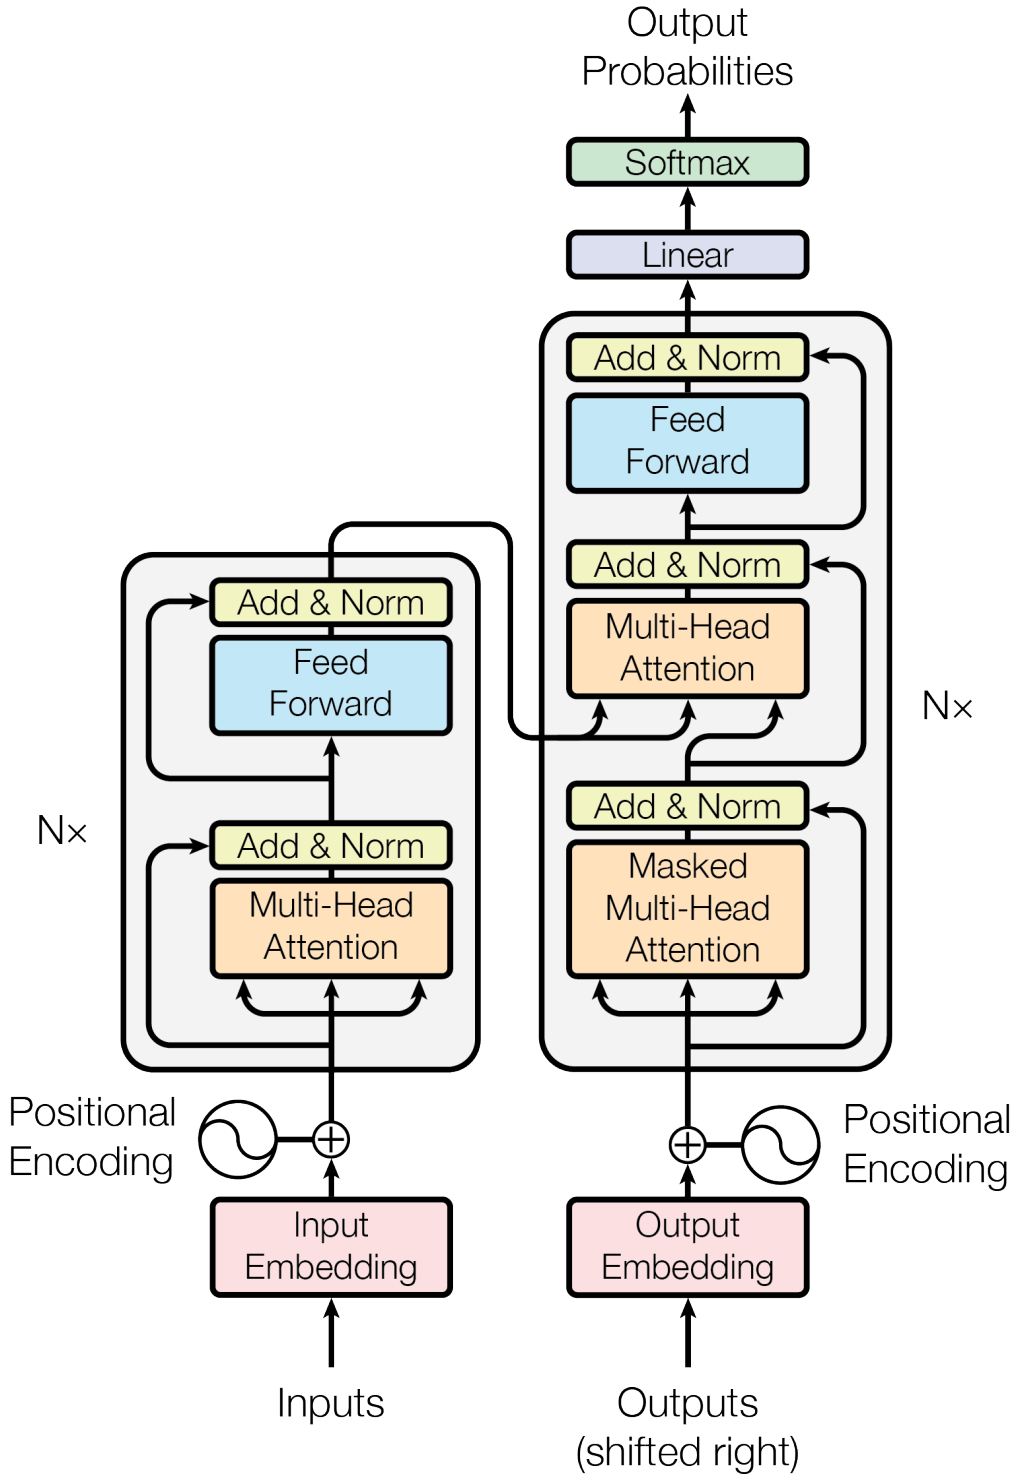
\includegraphics[width=0.5\textwidth]{Transformer model diagram}
\caption{Diagram depicting the architecture of the transformer model from \citet{AttentionIsAllYouNeed}.}
\end{figure}
\subsection{Problems solved by transformers}
The point of transformers was to overcome the problems faced by the previous state-of-the-art architectures while still including prominent aspects of the RNN and Convolutional Neural Network (CNN) models.

The RNN model has two notable weaknesses. First is its inability to learn long-term patterns, due to the exploding and vanishing gradient problems that occur during backpropagation.
Secondly, its recurrent connection is also a weakness. This is because it is not possible to compute the cell at time step $i$ until the cell at time step $i-1$ has been computed as information is propagated along a sequence.

In contrast, one of the benefits of CNNs is that they can be computed concurrently. However, unlike RNNs, they are unable to learn even short-term patterns. The size of the patterns they can learn is limited by their architecture.

Transformers attempt to feature the best of both techniques.
Transformers can model dependencies over the whole range of the input sequence as easily they can model neighboring sequences. And there are no recurrent connections, allowing efficient computation using parallelization. This is facilitated through the use of the self-attention mechanism.\cite{TransformersScratchPeterbloem}


\subsection{Self-attention Mechanism}
A self-attention mechanism is a sequence to sequence operation. This means that the input is a sequence of vectors $x_{1},x_{2},\ldots, x_{t}$, and the output is also a sequence of vectors $y_{1},y_{2},\ldots, y_{t}$.
These vectors all have dimension $k$.

To get the output vector $y_{i}$, the operation takes a weighted average over all input vectors.
$$
y_{i}=\sum_{j}w_{ij}x_{j}
$$
Here, $j$ indexes over the whole sequence, and the sum of all the weights in the sequence is one.
The weight $w_{ij}$ is derived from a function over $x_{i}$ and $x_{j}$.
This could, for example, be the dot product:
$$
w'_{ij}=x_{i}^Tx_{j}
$$
where $x_{i}$ is the input vector at the same position as the current output vector $y_{i}$.
The next output vector has a completely different series of dot products, and therefore a different weighted sum.

As the dot product can result in values between negative and positive infinity, the softmax activation function is used to map values to the interval $[0,1]$, and to ensure that they sum to $1$ over the entire sequence:
$$
w_{ij}=\frac{e^{w'_{ij}}}{\sum_{j}e^{w'_{ij}}}
$$
For maximum efficiency, computations are vectorized as much as possible. The resulting calculations become:
\begin{gather}
W'=X^TX\\
W=\text{softmax}(W')\\
Y^T=WX^T
\end{gather}\cite{TransformersScratchPeterbloem}


\subsection{How transformers work}
Transformers, as mentioned, primarily use self-attention. This forms the basis of the architecture.

There are several different variations of the transformer architecture, and the following is just one such variant.

First, the transformer block applies self-attention. Then it does layer normalization, after which it applies a feed forward network. The feed forward network here is a single MLP applied independently to each vector. And lastly, another layer normalization is applied.

The network may become permutation invariant, meaning the output will not change despite reordering. In the context of natural language processing, the ordering of the words in the input sentence would not matter. This can be detrimental to the training process, as it means the model is not learning the dependencies between words---positions matter. If every word in this paper were ordered alphabetically, it would not make much sense.

To solve this, one can use positional embeddings or positional encodings.

With positional embedding, the position of the word in the sentence is embedded. For this to work during training, sequences of every length would need to be seen, otherwise, the relevant positional embeddings do not get trained.

Positional encodings work in a similar fashion, except the positional vectors are not learned.
Instead, a function is chosen $f:\mathbb{N}\rightarrow\mathbb{R}^k$ that maps the positions to real-valued vectors. The network is left to figure out how to interpret these.\cite{TransformersScratchPeterbloem}